\documentclass[10pt,aspectratio=169,xcolor={table,dvipsnames}]{beamer}

% ==============================================================================
% THEME & COLOR CONFIGURATION (USMS & FST Béni Mellal Identity)
% ==============================================================================
\usetheme{Madrid}
\usecolortheme{default}

% Academic Color Palette
\definecolor{NavyBlue}{RGB}{11, 37, 69}       % Primary USMS Navy
\definecolor{SlateBlue}{RGB}{20, 60, 110}     % Secondary Academic Blue
\definecolor{TealAccent}{RGB}{0, 128, 128}    % Highlight Accent
\definecolor{AmberAlert}{RGB}{192, 57, 43}    % Warning / Alert
\definecolor{SuccessGreen}{RGB}{39, 174, 96}  % Good results
\definecolor{LightGrayBg}{RGB}{245, 247, 250} % Block background
\definecolor{BorderGray}{RGB}{218, 225, 233}  % Subtle border

% Apply Palette to Beamer Elements
\setbeamercolor{palette primary}{bg=NavyBlue, fg=white}
\setbeamercolor{palette secondary}{bg=SlateBlue, fg=white}
\setbeamercolor{palette tertiary}{bg=NavyBlue!90, fg=white}
\setbeamercolor{structure}{fg=NavyBlue}
\setbeamercolor{title}{bg=NavyBlue, fg=white}
\setbeamercolor{frametitle}{bg=NavyBlue, fg=white}
\setbeamercolor{item}{fg=SlateBlue}
\setbeamercolor{block title}{bg=NavyBlue!15, fg=NavyBlue}
\setbeamercolor{block body}{bg=LightGrayBg, fg=black}
\setbeamercolor{block title alerted}{bg=AmberAlert!15, fg=AmberAlert}
\setbeamercolor{block body alerted}{bg=LightGrayBg, fg=black}
\setbeamercolor{block title example}{bg=SuccessGreen!15, fg=SuccessGreen}
\setbeamercolor{block body example}{bg=LightGrayBg, fg=black}

% Clean up navigation & enhance footline (strictly without author names)
\setbeamertemplate{navigation symbols}{}
\setbeamertemplate{footline}{
  \leavevmode%
  \hbox{%
    \begin{beamercolorbox}[wd=.333333\paperwidth,ht=2.5ex,dp=1.1ex,left,leftskip=1em]{author in head/foot}%
      \usebeamerfont{author in head/foot}(Session C01-2)
    \end{beamercolorbox}%
    \begin{beamercolorbox}[wd=.333333\paperwidth,ht=2.5ex,dp=1.1ex,center]{title in head/foot}%
      \usebeamerfont{title in head/foot}Recurrence Risk in OSCC
    \end{beamercolorbox}%
    \begin{beamercolorbox}[wd=.333333\paperwidth,ht=2.5ex,dp=1.1ex,right,rightskip=1em]{date in head/foot}%
      \usebeamerfont{date in head/foot}FSTBM -- 14 Nov 2026 \quad \textbf{\insertframenumber{} / \inserttotalframenumber}
    \end{beamercolorbox}%
  }%
  \vskip0pt%
}

% ==============================================================================
% PACKAGES & MATH DEFINITIONS (Universal Compatibility: pdflatex / xelatex / lualatex)
% ==============================================================================
\usepackage{iftex}
\ifPDFTeX
  \usepackage[utf8]{inputenc}
  \usepackage[T1]{fontenc}
  \usepackage{lmodern}
\fi
\usepackage{booktabs}
\usepackage{graphicx}
\graphicspath{{./}{report/}{figures/}}
\usepackage{amsmath,amssymb}
\usepackage{tikz}

% Project Math Macros
\newcommand{\ROC}{\text{ROC-AUC}}
\newcommand{\AUPRC}{\text{AUPRC}}
\newcommand{\Brier}{\text{Brier}}
\newcommand{\aOR}{\text{aOR}}
\newcommand{\CI}{\text{CI}}
\newcommand{\RF}{\text{RF}}
\newcommand{\LR}{\text{LR}}

% ==============================================================================
% METADATA
% ==============================================================================
\title[Recurrence Risk in OSCC]{From Clinical Characteristics to Surgical Pathology}
\subtitle{Statistical and Machine-Learning Analysis of Recurrence Risk in Oral Squamous Cell Carcinoma}

\author[Session C01-2]{%
  Yassine Oulhammous \and Mahdi Boughrous \and Yasmine Elasri \and Mohamed Taha Benhassoun \and Mustapha Amarzoug%
}

\institute[USMS - FSTBM]{
  Master / Doctoral Program -- Modules: Statistics \& Data Analysis\\
  \textbf{Faculty of Sciences and Techniques of Béni Mellal (FSTBM)}\\
  Sultan Moulay Slimane University, Morocco\\[0.2cm]
  \textit{Supervised by:} \textbf{Prof.~Aziz OUHINOU} \& \textbf{Prof.~Hicham MOUSSA}
}

\date{Saturday, November 14, 2026}

% ==============================================================================
% DOCUMENT BODY
% ==============================================================================
\begin{document}

% ------------------------------------------------------------------------------
% SLIDE 1: TITLE SLIDE (0:00 - 0:45)
% ------------------------------------------------------------------------------
\begin{frame}[plain]
  \vspace{0.2cm}
  \begin{columns}[c]
    \column{0.20\textwidth}
      \centering
      
\includegraphics[height=1.4cm]{logo.png}
    \column{0.80\textwidth}
      \centering
      {\scriptsize \textbf{SULTAN MOULAY SLIMANE UNIVERSITY} -- FACULTY OF SCIENCES AND TECHNIQUES BÉNI MELLAL}\\
      {\tiny Final Evaluation: Statistics \& Data Analysis Modules $\cdot$ Oral Defense -- Session C01-2}
  \end{columns}
  
  \vspace{0.3cm}
  \begin{centering}
    \begin{beamercolorbox}[sep=6pt,center,rounded=true,shadow=true]{title}
      {\fontsize{13}{16}\selectfont\textbf{From Clinical Characteristics to Surgical Pathology}}\\[0.15cm]
      {\fontsize{9.5}{12}\selectfont Statistical and Machine-Learning Analysis of Recurrence Risk in OSCC}
    \end{beamercolorbox}
  \end{centering}

  \vspace{0.35cm}
  \begin{columns}[t]
    \column{0.56\textwidth}
      \textbf{\scriptsize Research Team \& Specializations:}
      \begin{itemize}\setlength{\itemsep}{1pt}
        \item {\tiny \textbf{Yassine Oulhammous} -- Artificial Intelligence (Lab. TIAD)}
        \item {\tiny \textbf{Mahdi Boughrous} -- Artificial Intelligence (Lab. TIAD)}
        \item {\tiny \textbf{Yasmine Elasri} -- Mathematics (Lab. MPA)}
        \item {\tiny \textbf{Mohamed Taha Benhassoun} -- Biology}
        \item {\tiny \textbf{Mustapha Amarzoug} -- Organic Chemistry (Lab. 3BIO)}
      \end{itemize}
    \column{0.44\textwidth}
      \textbf{\scriptsize Academic Supervision:}
      \begin{itemize}\setlength{\itemsep}{2pt}
        \item {\tiny \textbf{Prof.~Aziz OUHINOU}}
        \item {\tiny \textbf{Prof.~Hicham MOUSSA}}
      \end{itemize}
      \vspace{0.25cm}
      \begin{block}{\scriptsize Academic Institution}
        {\tiny Department of Mathematics \& Informatics\\Faculty of Sciences and Techniques of Béni Mellal}
      \end{block}
  \end{columns}
\end{frame}

% ------------------------------------------------------------------------------
% SLIDE 2: CLINICAL CONTEXT & THE TIMELINE PARADOX (0:45 - 1:45)
% ------------------------------------------------------------------------------
\begin{frame}{Clinical Context \& The Temporal Problem}
  \begin{columns}[c]
    \column{0.55\textwidth}
      \begin{block}{Epidemiological Stature of OSCC}
        \begin{itemize}\setlength{\itemsep}{3pt}
          \item \textbf{Oral Squamous Cell Carcinoma (OSCC)}: $>90\%$ of all oral cavity malignancies ($\sim$377,000 cases, 177,000 deaths/year).
          \item \textbf{2-Year Post-Surgical Recurrence}: Major determinant of morbidity, intensive surveillance, and mortality.
        \end{itemize}
      \end{block}

      \begin{alertblock}{The Core Methodological Trap: Data Timing}
        \begin{itemize}\setlength{\itemsep}{2pt}
          \item Clinical features (demographics, habits, systemic diseases) exist \textbf{before surgery}.
          \item Histopathology (tumor differentiation, invasion, embolus) is obtained \textbf{only after surgical resection}.
          \item \textit{Pre-treatment prediction cannot legally claim post-operative surgical markers!}
        \end{itemize}
      \end{alertblock}

    \column{0.45\textwidth}
      \centering
      \begin{beamercolorbox}[sep=8pt,rounded=true,center]{block body}
        \textbf{\footnotesize The Clinical Information Timeline}\\[0.3cm]
        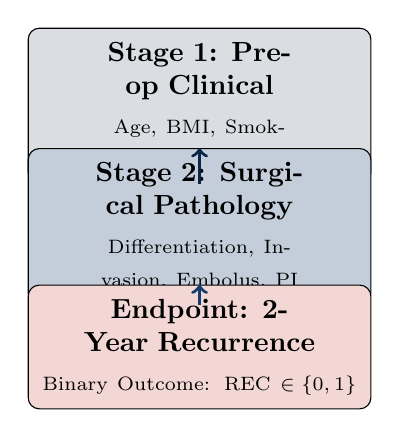
\begin{tikzpicture}[scale=0.85]
          \node[draw, rounded corners, fill=NavyBlue!15, text width=4.0cm, align=center, inner sep=5pt] at (0, 1.8) (t1) 
            {\textbf{Stage 1: Pre-op Clinical}\\[2pt]{\scriptsize Age, BMI, Smoking, Comorbidities}};
          \node[draw, rounded corners, fill=SlateBlue!25, text width=4.0cm, align=center, inner sep=5pt] at (0, 0) (t2) 
            {\textbf{Stage 2: Surgical Pathology}\\[2pt]{\scriptsize Differentiation, Invasion, Embolus, PI}};
          \node[draw, rounded corners, fill=AmberAlert!20, text width=4.0cm, align=center, inner sep=5pt] at (0, -1.8) (t3) 
            {\textbf{Endpoint: 2-Year Recurrence}\\[2pt]{\scriptsize Binary Outcome: REC $\in \{0, 1\}$}};
          
          \draw[->, very thick, NavyBlue] (t1) -- (t2);
          \draw[->, very thick, SlateBlue] (t2) -- (t3);
        \end{tikzpicture}
      \end{beamercolorbox}
  \end{columns}
\end{frame}

% ------------------------------------------------------------------------------
% SLIDE 3: RESEARCH QUESTIONS & METHODOLOGY FLOW (1:45 - 2:30)
% ------------------------------------------------------------------------------
\begin{frame}{Research Questions \& Dual-Perspective Design}
  \vspace{-0.1cm}
  \begin{beamercolorbox}[sep=4pt,rounded=true,center]{block title}
    \textbf{Three Sequential Scientific Questions}
  \end{beamercolorbox}
  \vspace{0.15cm}

  \begin{columns}[t]
    \column{0.32\textwidth}
      \begin{block}{\centering \small 1. Clinical Association}
        \vspace{0.1cm}
        {\scriptsize Do patient-level lifestyle, demographic, and comorbidity factors predict 2-year recurrence?}
        \begin{itemize}\setlength{\itemsep}{0pt}
          \item {\tiny Mann--Whitney $U$ tests}
          \item {\tiny Pearson $\chi^2$ \& Cramér's $V$}
        \end{itemize}
      \end{block}

    \column{0.32\textwidth}
      \begin{block}{\centering \small 2. Pathology Independence}
        \vspace{0.1cm}
        {\scriptsize Does surgical pathology provide independent signal after adjusting for baseline clinical factors?}
        \begin{itemize}\setlength{\itemsep}{0pt}
          \item {\tiny Multivariable Logistic Regression}
          \item {\tiny Adjusted Odds Ratios ($\aOR$)}
        \end{itemize}
      \end{block}

    \column{0.32\textwidth}
      \begin{block}{\centering \small 3. Predictive Generalization}
        \vspace{0.1cm}
        {\scriptsize Can ML models reliably generalize recurrence prediction to unseen, held-out patients?}
        \begin{itemize}\setlength{\itemsep}{0pt}
          \item {\tiny Regularized LR \& Random Forest}
          \item {\tiny $\ROC$, $\AUPRC$, Calibration, DCA}
        \end{itemize}
      \end{block}
  \end{columns}

  \vspace{0.25cm}
  \begin{exampleblock}{Methodological Principle: Inference vs. Prediction}
    \centering \small
    \textbf{Statistical Association} (explaining cohort patterns) $\;\neq\;$ \textbf{Machine Learning Prediction} (out-of-sample decision utility).
  \end{exampleblock}
\end{frame}

% ------------------------------------------------------------------------------
% SLIDE 4: COHORT, SPLIT INTEGRITY & LEAKAGE PREVENTION (2:30 - 3:30)
% ------------------------------------------------------------------------------
\begin{frame}{Cohort Architecture \& Leakage Prevention}
  \begin{columns}[c]
    \column{0.50\textwidth}
      \begin{block}{Multi-OSCC Benchmark Cohort ($N = 1,325$)}
        \begin{itemize}\setlength{\itemsep}{3pt}
          \item \textbf{Recurrence Events}: $n = 275$ ($20.75\%$ prevalence).
          \item \textbf{Non-Recurrence}: $n = 1,050$ ($79.25\%$).
          \item Severe class imbalance ($\sim 4:1$ ratio).
        \end{itemize}
      \end{block}

      \begin{alertblock}{Strict Leakage Prevention Protocol}
        \textbf{Excluded Post-Treatment Variables}:
        \begin{itemize}\setlength{\itemsep}{1pt}
          \item Surgical margins status \& flap reconstruction
          \item Post-op tracheostomy, adjuvant chemo/radiotherapy
          \item Recurrence-free interval \& follow-up duration
        \end{itemize}
        {\scriptsize $\implies$ Prevents trivial target leakage into predictors.}
      \end{alertblock}

    \column{0.50\textwidth}
      \begin{block}{Partitioning Integrity (\texttt{split\_seed=2024})}
        \centering
        \small
        \begin{tabular}{lccc}
          \toprule
          \textbf{Partition} & \textbf{Total ($N$)} & \textbf{Events} & \textbf{Prevalence} \\
          \midrule
          \textbf{Training}   & 925 & 226 & 24.43\% \\
          \textbf{Validation} & 200 & 45  & 22.50\% \\
          \textbf{Held-Out Test}& 200 & 49  & 24.50\% \\
          \midrule
          \textbf{Overall}    & 1,325 & 275 & 20.75\% \\
          \bottomrule
        \end{tabular}
      \end{block}

      \begin{exampleblock}{Feature Preprocessing Safeguards}
        \begin{itemize}\setlength{\itemsep}{1pt}
          \item Zero patient ID overlap across partitions.
          \item Preprocessing (median impute, scaling, one-hot encoding) fit \textbf{strictly on Train}.
          \item HPV excluded due to $22.4\%$ missingness.
        \end{itemize}
      \end{exampleblock}
  \end{columns}
\end{frame}

% ------------------------------------------------------------------------------
% SLIDE 5: EXPLORATORY STATISTICAL ASSOCIATIONS (3:30 - 4:30)
% ------------------------------------------------------------------------------
\begin{frame}{Baseline Statistical Associations ($N=1,325$)}
  \begin{columns}[c]
    \column{0.52\textwidth}
      \centering
      \scriptsize
      \setlength{\tabcolsep}{3pt}
      \begin{tabular*}{\linewidth}{@{\extracolsep{\fill}}lcccc@{}}
        \toprule
        \textbf{Variable} & \textbf{No Rec (0)} & \textbf{Rec (1)} & \textbf{Effect} & \textbf{$p$-value} \\
        \midrule
        Age (median [IQR]) & 59 [50--68] & 56 [47--65] & $\Delta=-3$ & \textbf{0.015} \\
        BMI (median [IQR]) & 22.5 [20--25] & 21.8 [20--25] & $\Delta=-0.7$ & \textbf{0.012} \\
        \midrule
        Smoking history    & 40.0\% & 37.1\% & $V=0.019$ & 0.487 \\
        Alcohol history    & 23.3\% & 22.2\% & $V=0.007$ & 0.797 \\
        Betel-nut history  & 6.3\%  & 6.9\%  & $V=0.007$ & 0.812 \\
        \midrule
        \rowcolor{NavyBlue!10}
        \textbf{Tumor Diff. (TD)} & & & $V=0.111$ & \textbf{$<0.001$} \\
        \quad Well (G1)    & 35.9\% & 26.5\% & -- & -- \\
        \quad Moderate (G2)& 52.0\% & 53.1\% & -- & -- \\
        \quad Poor (G3)    & 12.1\% & 20.4\% & -- & -- \\
        \rowcolor{NavyBlue!10}
        \textbf{Tumor Invasion (TI)} & 44.8\% & 53.8\% & $V=0.072$ & \textbf{0.009} \\
        \rowcolor{NavyBlue!10}
        \textbf{Cancer Embolus (CE)} & 7.5\%  & 12.0\% & $V=0.062$ & \textbf{0.024} \\
        \rowcolor{NavyBlue!10}
        \textbf{Perineural Inv. (PI)}& 16.8\% & 24.7\% & $V=0.081$ & \textbf{0.003} \\
        \bottomrule
      \end{tabular*}

    \column{0.48\textwidth}
      \begin{block}{Key Clinical Insight: Etiology $\neq$ Recurrence}
        \begin{itemize}\setlength{\itemsep}{2pt}
          \item \textbf{Counter-Intuitive Finding}: Lifestyle carcinogens (tobacco, alcohol, betel nut) show \textbf{no association} with recurrence ($p > 0.45$).
          \item \textit{Biological reason}: Habits induce primary oncogenesis, but recurrence after resection is dictated by \textbf{intrinsic tumor biology} and invasiveness.
        \end{itemize}
      \end{block}

      \begin{exampleblock}{Pathology Variables Dominate}
        \begin{itemize}\setlength{\itemsep}{2pt}
          \item All 4 surgical pathology markers (TD, TI, CE, PI) are highly significant in bivariate tests ($p < 0.05$).
        \end{itemize}
      \end{exampleblock}
  \end{columns}
\end{frame}

% ------------------------------------------------------------------------------
% SLIDE 6: MULTIVARIABLE LOGISTIC REGRESSION (4:30 - 5:30)
% ------------------------------------------------------------------------------
\begin{frame}{Multivariable Logistic Regression ($n=1,317$)}
  \begin{columns}[c]
    \column{0.48\textwidth}
      \centering
      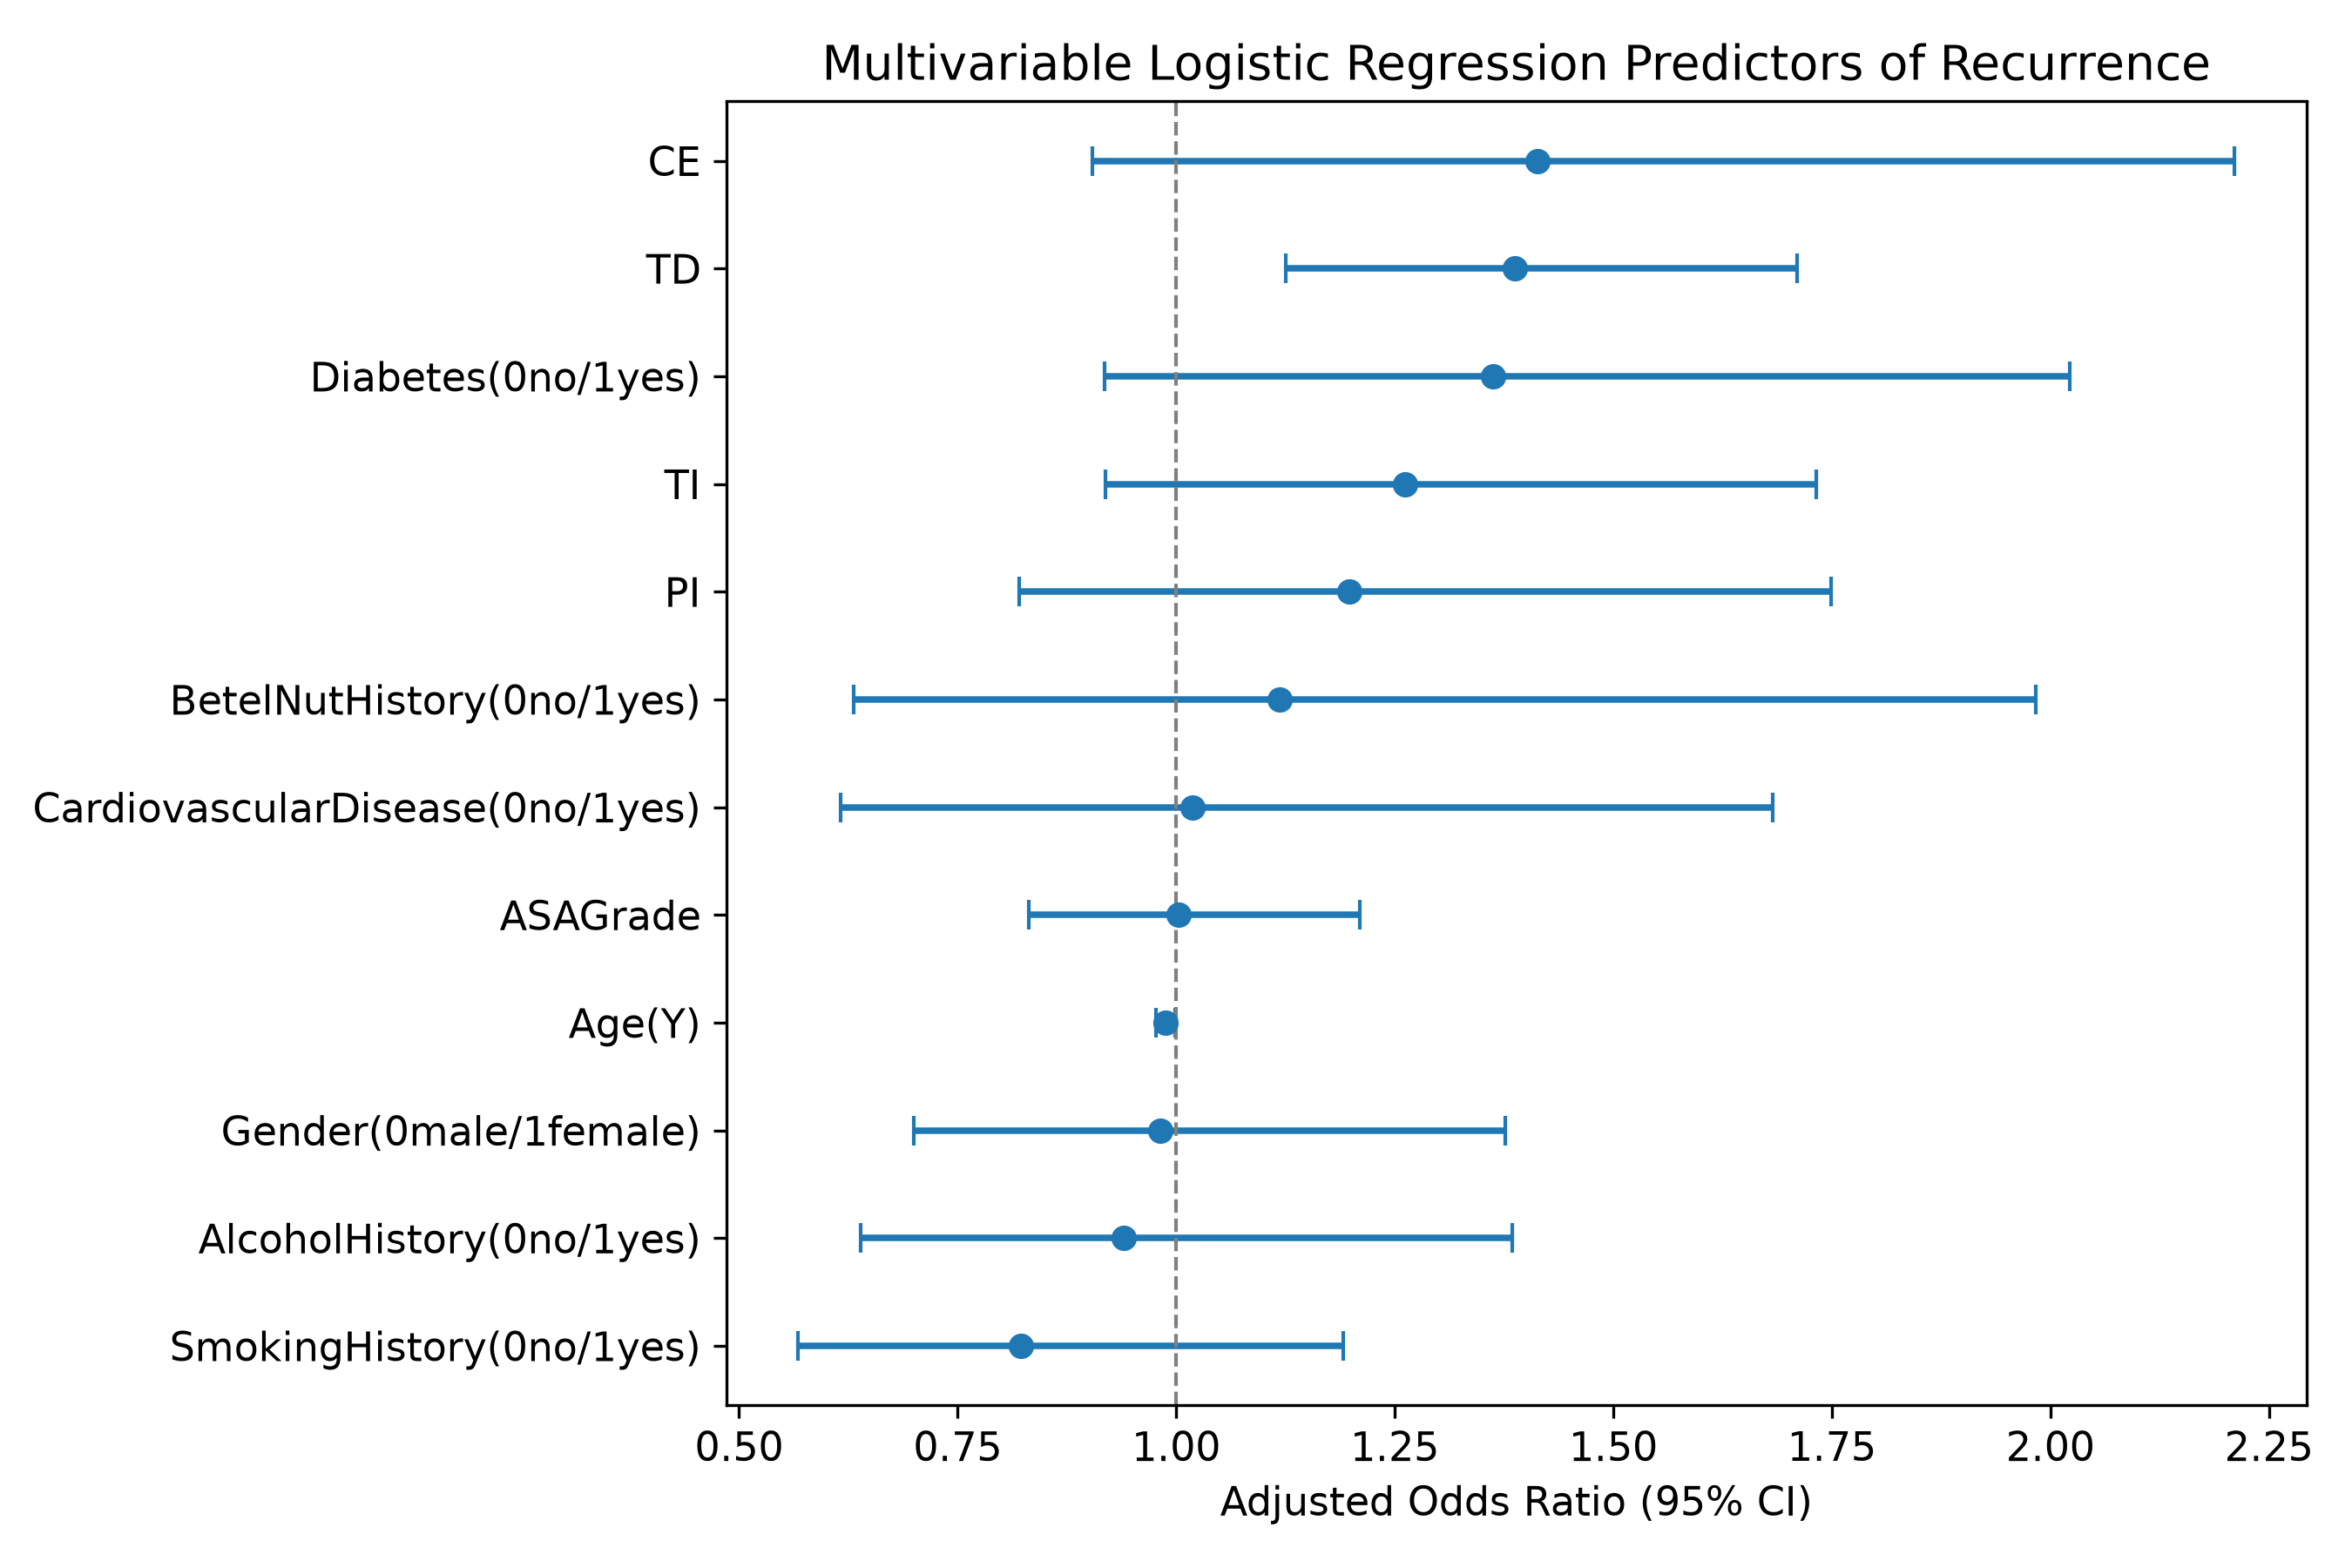
\includegraphics[width=\linewidth]{forest_plot_odds_ratios.png}

    \column{0.52\textwidth}
      \begin{block}{Adjusted Odds Ratios ($\aOR$, 95\% CI)}
        \centering
        \scriptsize
        \begin{tabular}{lccc}
          \toprule
          \textbf{Predictor} & \textbf{$\aOR$} & \textbf{95\% CI} & \textbf{$p$-value} \\
          \midrule
          Age (per year)         & 0.988 & [0.977, 0.999] & \textbf{0.0306} \\
          Smoking history        & 0.822 & [0.568, 1.191] & 0.3012 \\
          Alcohol history        & 0.940 & [0.639, 1.384] & 0.7545 \\
          Betel-nut history      & 1.119 & [0.631, 1.983] & 0.7013 \\
          \midrule
          \rowcolor{SuccessGreen!15}
          \textbf{Tumor Diff. (TD)} & \textbf{1.387} & \textbf{[1.125, 1.711]} & \textbf{0.0022} \\
          Tumor Invasion (TI)    & 1.262 & [0.919, 1.732] & 0.1499 \\
          Cancer Embolus (CE)    & 1.413 & [0.904, 2.211] & 0.1294 \\
          Perineural Inv. (PI)   & 1.198 & [0.820, 1.749] & 0.3501 \\
          \bottomrule
        \end{tabular}
      \end{block}

      \begin{alertblock}{Critical Synthesis: TD Alone Persists}
        \begin{itemize}\setlength{\itemsep}{1pt}
          \item \textbf{Tumor Differentiation} is the \textbf{only} pathological factor that survives adjustment: $+38.7\%$ odds of recurrence per grade worsening.
          \item TI, CE, and PI attenuate once TD and clinical covariates are controlled for.
        \end{itemize}
      \end{alertblock}
  \end{columns}
\end{frame}

% ------------------------------------------------------------------------------
% SLIDE 7: MACHINE LEARNING PIPELINE & MODELING SETUP (5:30 - 6:15)
% ------------------------------------------------------------------------------
\begin{frame}{Machine Learning Setup: 3 Feature Configurations}
  \begin{columns}[t]
    \column{0.32\textwidth}
      \begin{block}{\centering \small Clinical-Only}
        \vspace{0.1cm}
        \begin{itemize}\setlength{\itemsep}{2pt}
          \item {\tiny 11 raw patient attributes}
          \item {\tiny Age, BMI, sex, habits, ASA grade, comorbidities, site}
          \item \textbf{\scriptsize 27 features} {\tiny post one-hot encoding}
          \item {\tiny Represents early pre-op baseline}
        \end{itemize}
      \end{block}

    \column{0.32\textwidth}
      \begin{block}{\centering \small Pathology-Only}
        \vspace{0.1cm}
        \begin{itemize}\setlength{\itemsep}{2pt}
          \item {\tiny 4 surgical pathology factors}
          \item {\tiny TD, TI, CE, PI}
          \item \textbf{\scriptsize 9 features} {\tiny post one-hot encoding}
          \item {\tiny Represents post-resection tumor biology}
        \end{itemize}
      \end{block}

    \column{0.32\textwidth}
      \begin{block}{\centering \small Combined Union}
        \vspace{0.1cm}
        \begin{itemize}\setlength{\itemsep}{2pt}
          \item {\tiny Full integration of both stages}
          \item \textbf{\scriptsize 36 features} {\tiny post one-hot encoding}
          \item {\tiny Tests whether clinical data adds incremental value}
        \end{itemize}
      \end{block}
  \end{columns}

  \vspace{0.25cm}
  \begin{columns}[c]
    \column{0.50\textwidth}
      \begin{exampleblock}{Algorithms Evaluated}
        \begin{itemize}\setlength{\itemsep}{2pt}
          \item \textbf{$L_2$-Regularized Logistic Regression (LR)}: Linear baseline with balanced weights.
          \item \textbf{Random Forest (RF)}: 200 estimators, max depth 4, balanced class weighting to handle 4:1 imbalance.
        \end{itemize}
      \end{exampleblock}

    \column{0.50\textwidth}
      \begin{alertblock}{Validation \& Tuning Safeguards}
        \begin{itemize}\setlength{\itemsep}{2pt}
          \item Decision thresholds tuned \textbf{only} on Validation set ($n=200$) via F1 maximization.
          \item Test set ($n=200$) evaluated strictly \textbf{once} as held-out evidence.
        \end{itemize}
      \end{alertblock}
  \end{columns}
\end{frame}

% ------------------------------------------------------------------------------
% SLIDE 8: PREDICTIVE PERFORMANCE & ROC ANALYSIS (6:15 - 7:30)
% ------------------------------------------------------------------------------
\begin{frame}{Held-Out Test Set Performance ($n=200$; 49 Events)}
  \begin{columns}[c]
    \column{0.52\textwidth}
      \centering
      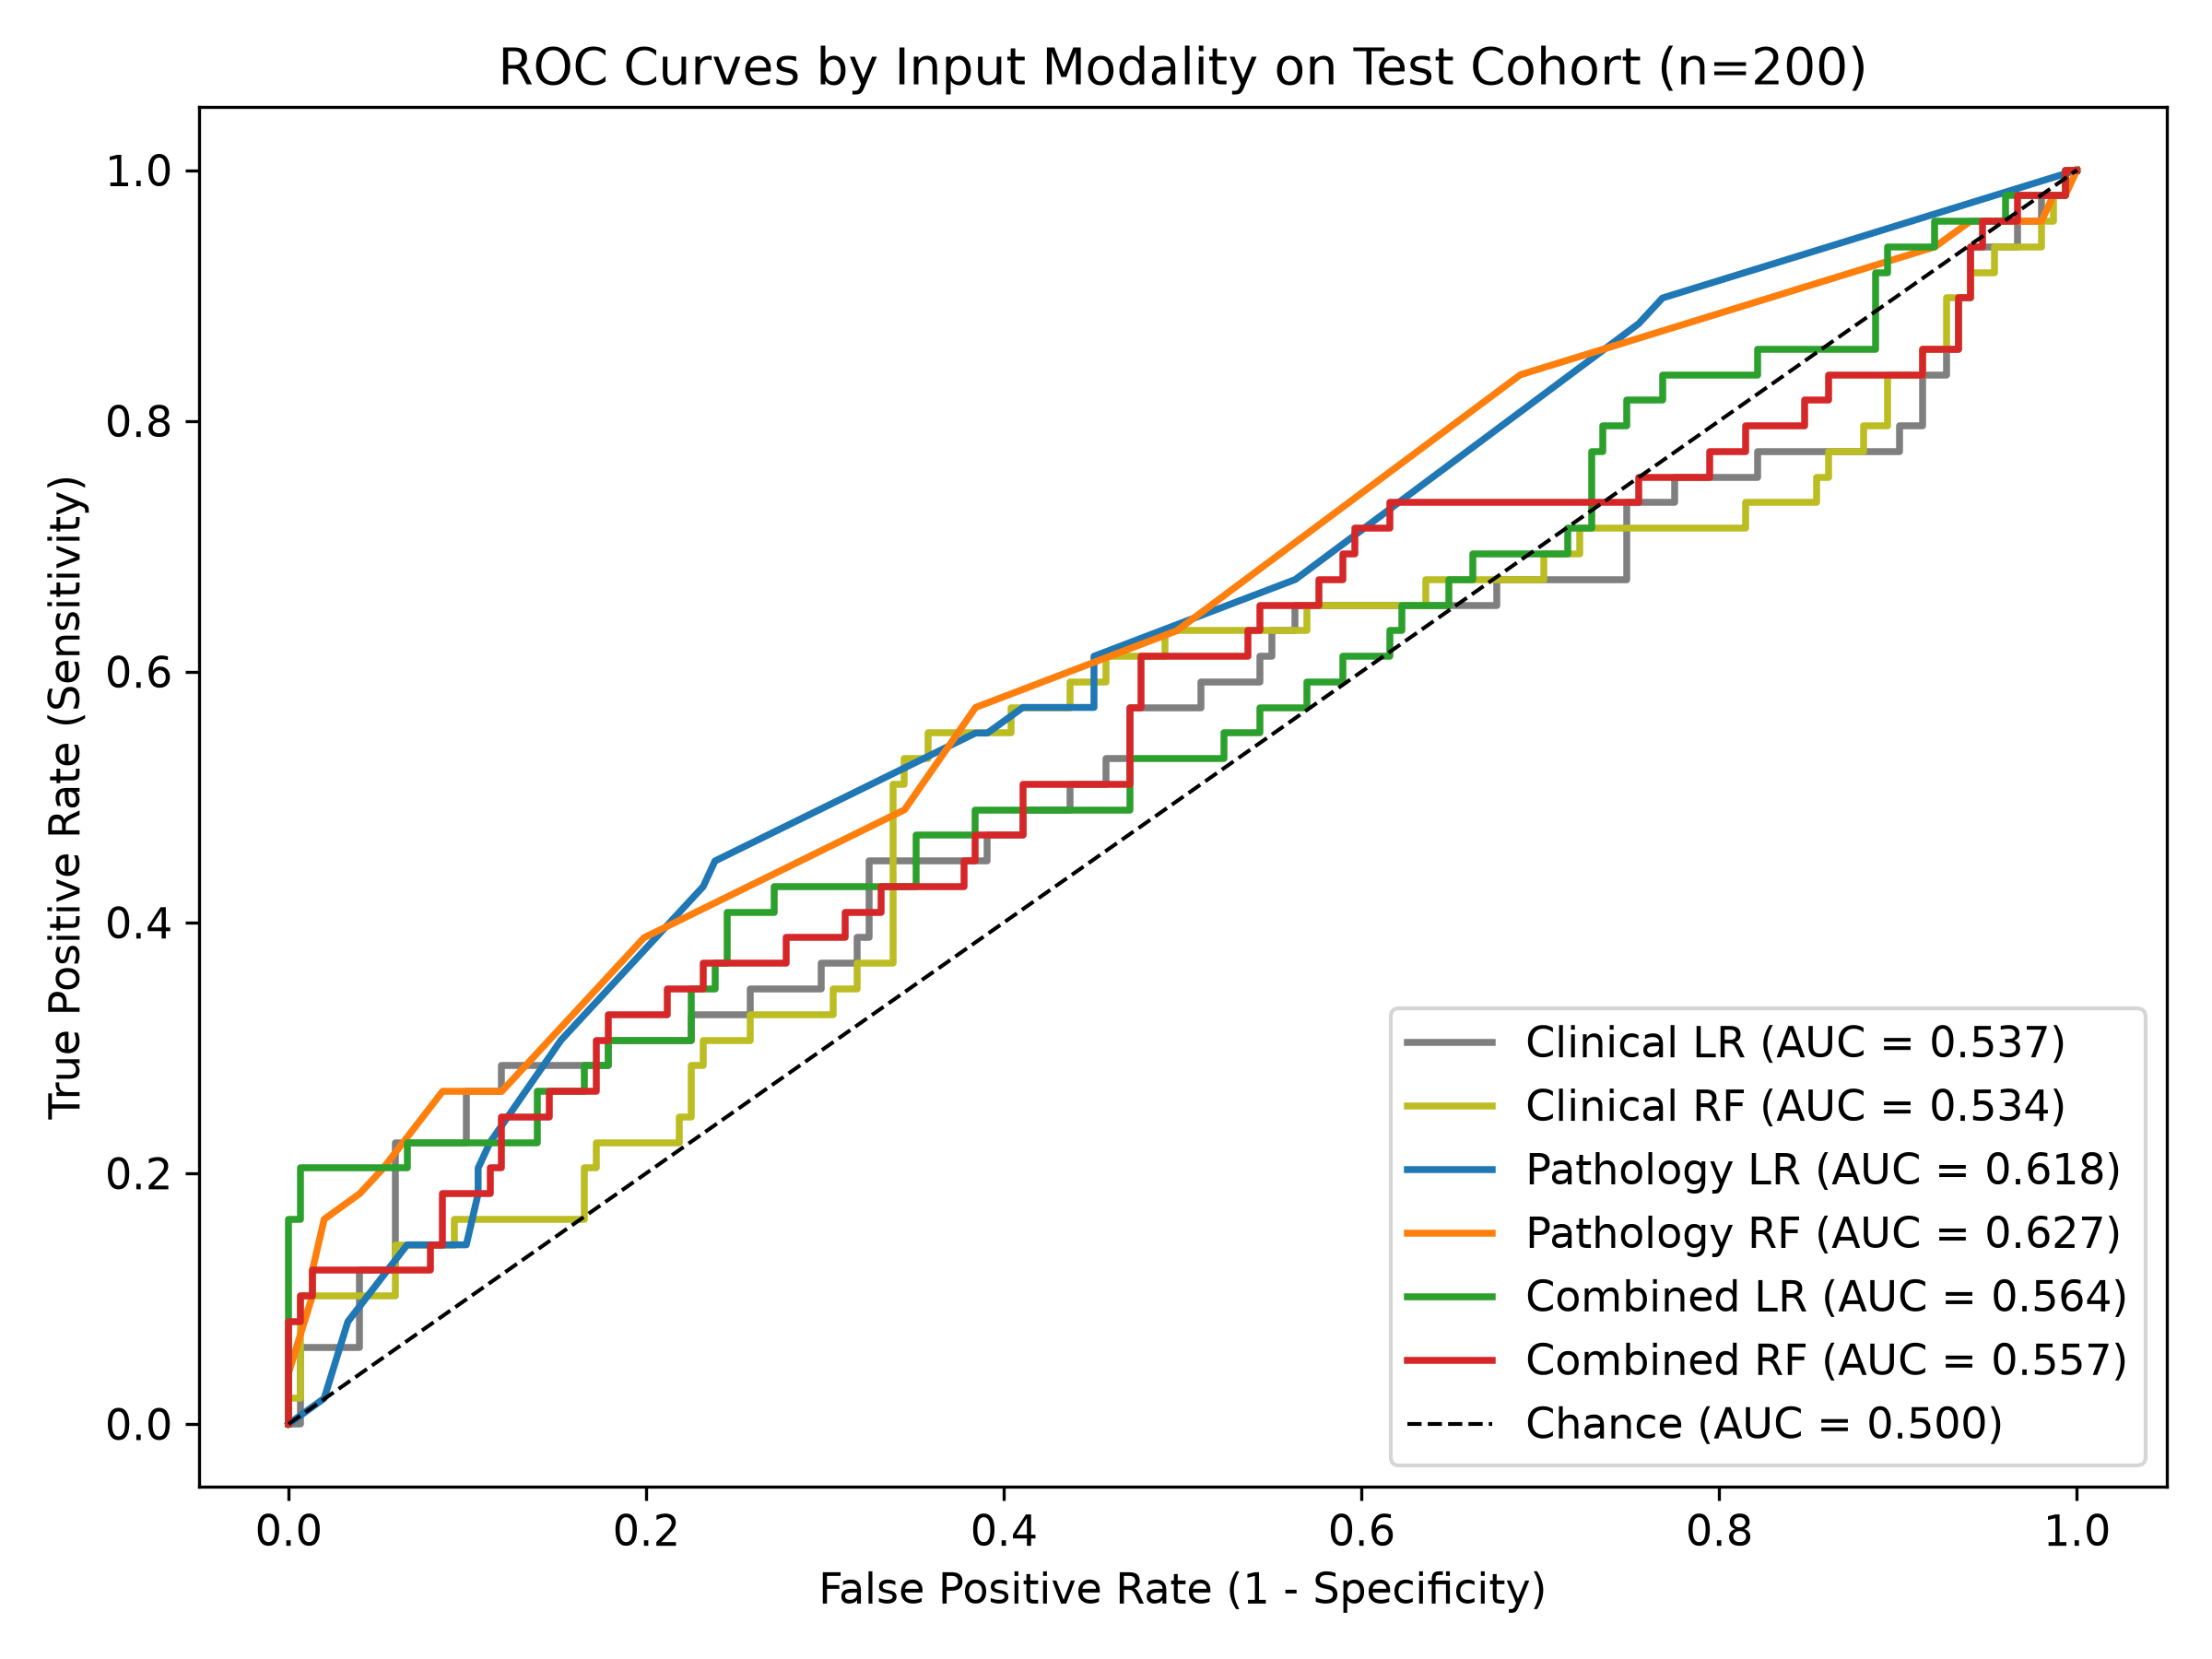
\includegraphics[width=\linewidth]{roc_curves.png}

    \column{0.48\textwidth}
      \centering
      \scriptsize
      \setlength{\tabcolsep}{2.5pt}
      \begin{tabular*}{\linewidth}{@{\extracolsep{\fill}}lccccc@{}}
        \toprule
        \textbf{Model} & \textbf{Config} & \textbf{$\ROC$} & \textbf{$\AUPRC$} & \textbf{F1} & \textbf{Recall} \\
        \midrule
        LR & Clinical   & 0.537 & 0.333 & 0.371 & 0.571 \\
        RF & Clinical   & 0.534 & 0.334 & 0.415 & 0.551 \\
        \midrule
        LR & Pathology  & 0.618 & 0.329 & 0.386 & 0.571 \\
        \rowcolor{SuccessGreen!15}
        \textbf{RF} & \textbf{Pathology} & \textbf{0.627} & 0.406 & \textbf{0.400} & \textbf{0.633} \\
        \midrule
        LR & Combined   & 0.564 & \textbf{0.429} & 0.340 & 0.490 \\
        RF & Combined   & 0.557 & 0.373 & 0.347 & 0.429 \\
        \bottomrule
      \end{tabular*}

      \vspace{0.2cm}
      \begin{block}{\scriptsize Key Takeaways from Test Set}
        \begin{itemize}\setlength{\itemsep}{1pt}
          \item {\tiny \textbf{Clinical-only} has near-chance discrimination ($\ROC \approx 0.535$).}
          \item {\tiny \textbf{Pathology-only RF} achieved highest discrimination ($\ROC = \mathbf{0.627}$, 95\% CI: $[0.528, 0.724]$).}
          \item {\tiny \textbf{Feature Dilation}: Adding 27 clinical features to pathology \textit{degraded} RF AUC from 0.627 to 0.557 (noise injection).}
        \end{itemize}
      \end{block}
  \end{columns}
\end{frame}

% ------------------------------------------------------------------------------
% SLIDE 9: CALIBRATION & THE THRESHOLD TRADEOFF (7:30 - 8:30)
% ------------------------------------------------------------------------------
\begin{frame}{Calibration \& The Operational Threshold Dilemma}
  \begin{columns}[c]
    \column{0.50\textwidth}
      \centering
      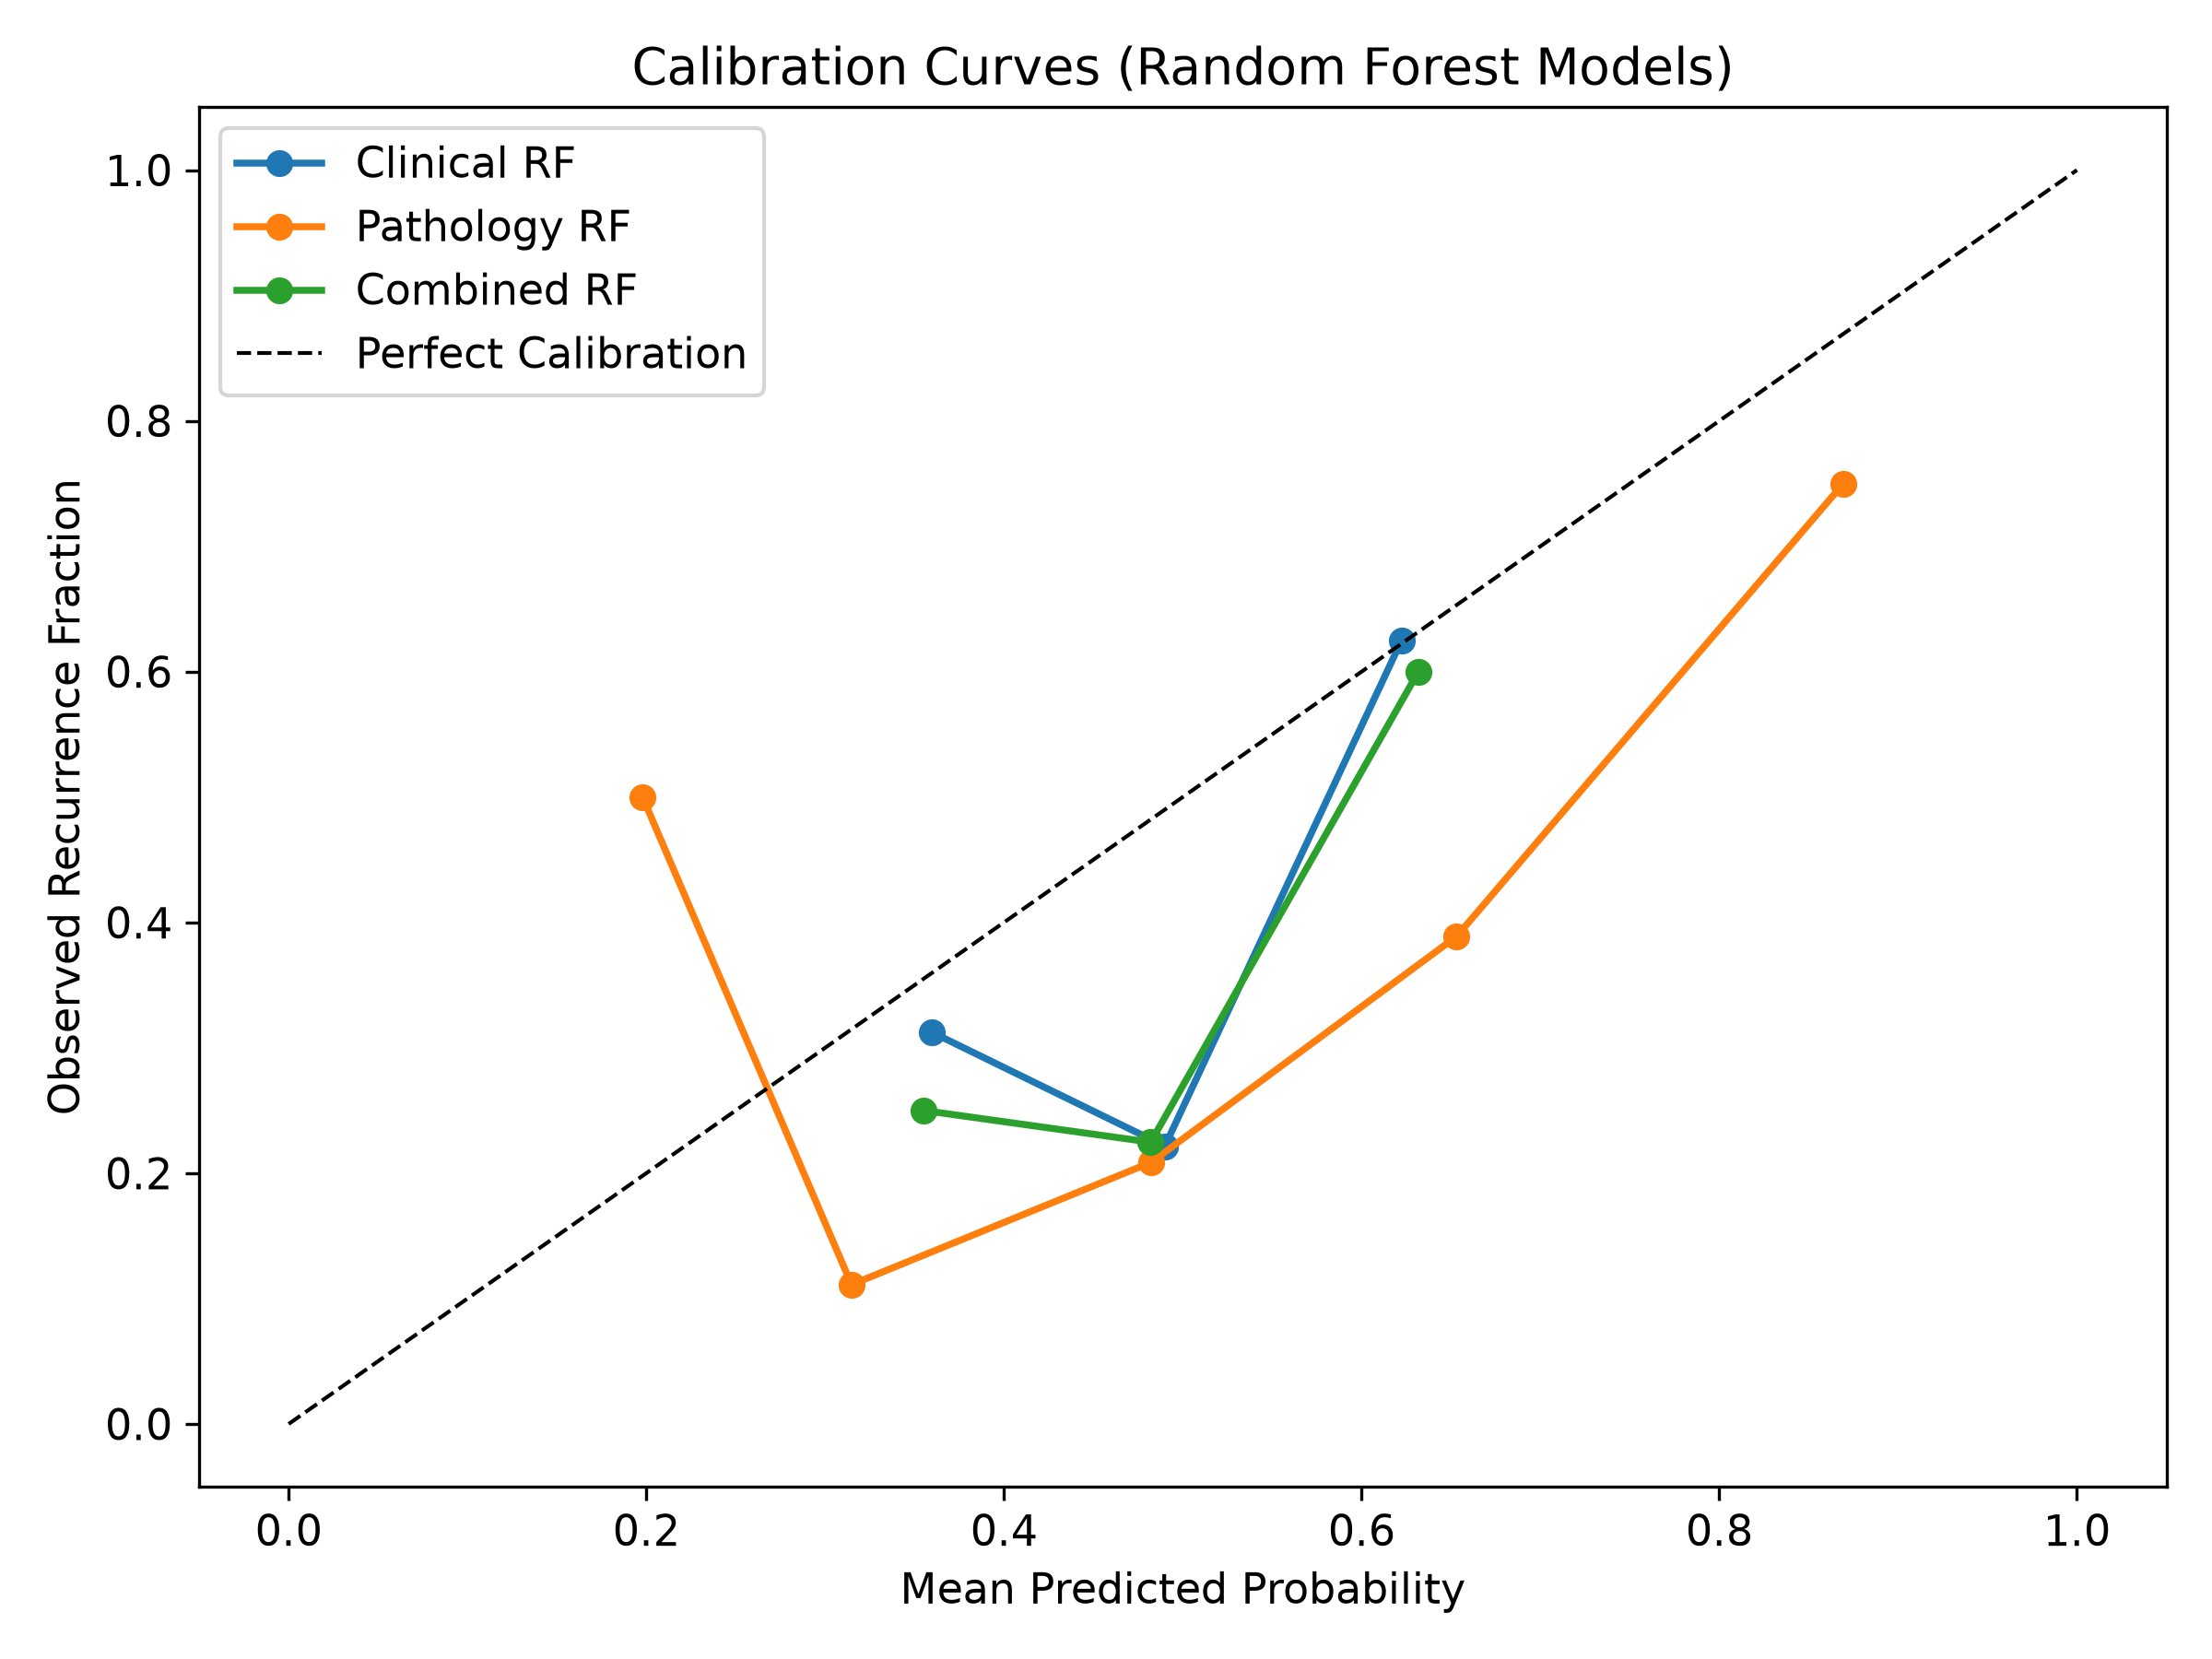
\includegraphics[width=\linewidth]{calibration_curves.png}

    \column{0.50\textwidth}
      \begin{alertblock}{Probabilistic Distortion: The Brier Paradox}
        \begin{itemize}\setlength{\itemsep}{2pt}
          \item \textbf{Null Brier Benchmark}: $p(1-p) = \mathbf{0.185}$.
          \item Model Briers ($0.239 - 0.259$) are \textbf{worse} than null!
          \item \textit{Why?} Balanced class weighting artificially boosted positive prevalence during training $\implies$ calibration intercept $\approx -1.1$ (systematic probability overestimation).
        \end{itemize}
      \end{alertblock}

      \begin{block}{Threshold Selection Trade-off (Pathology RF)}
        \centering
        \scriptsize
        \begin{tabular}{lcccc}
          \toprule
          \textbf{Threshold} & \textbf{Recall} & \textbf{Spec.} & \textbf{TP} & \textbf{FP} \\
          \midrule
          Default ($\tau = 0.50$)   & 63.3\% & 50.3\% & 31/49 & 75/151 \\
          Val-Opt ($\tau = 0.453$)  & \textbf{83.7\%} & \textbf{31.1\%} & \textbf{41/49} & \textbf{104/151} \\
          \bottomrule
        \end{tabular}
        \vspace{0.1cm}\\
        {\tiny Gaining 10 true recurrences costs 29 additional false alarms!}
      \end{block}
  \end{columns}
\end{frame}

% ------------------------------------------------------------------------------
% SLIDE 10: DECISION CURVE ANALYSIS (DCA) (8:30 - 9:15)
% ------------------------------------------------------------------------------
\begin{frame}{Clinical Utility: Decision Curve Analysis (DCA)}
  \begin{columns}[c]
    \column{0.52\textwidth}
      \centering
      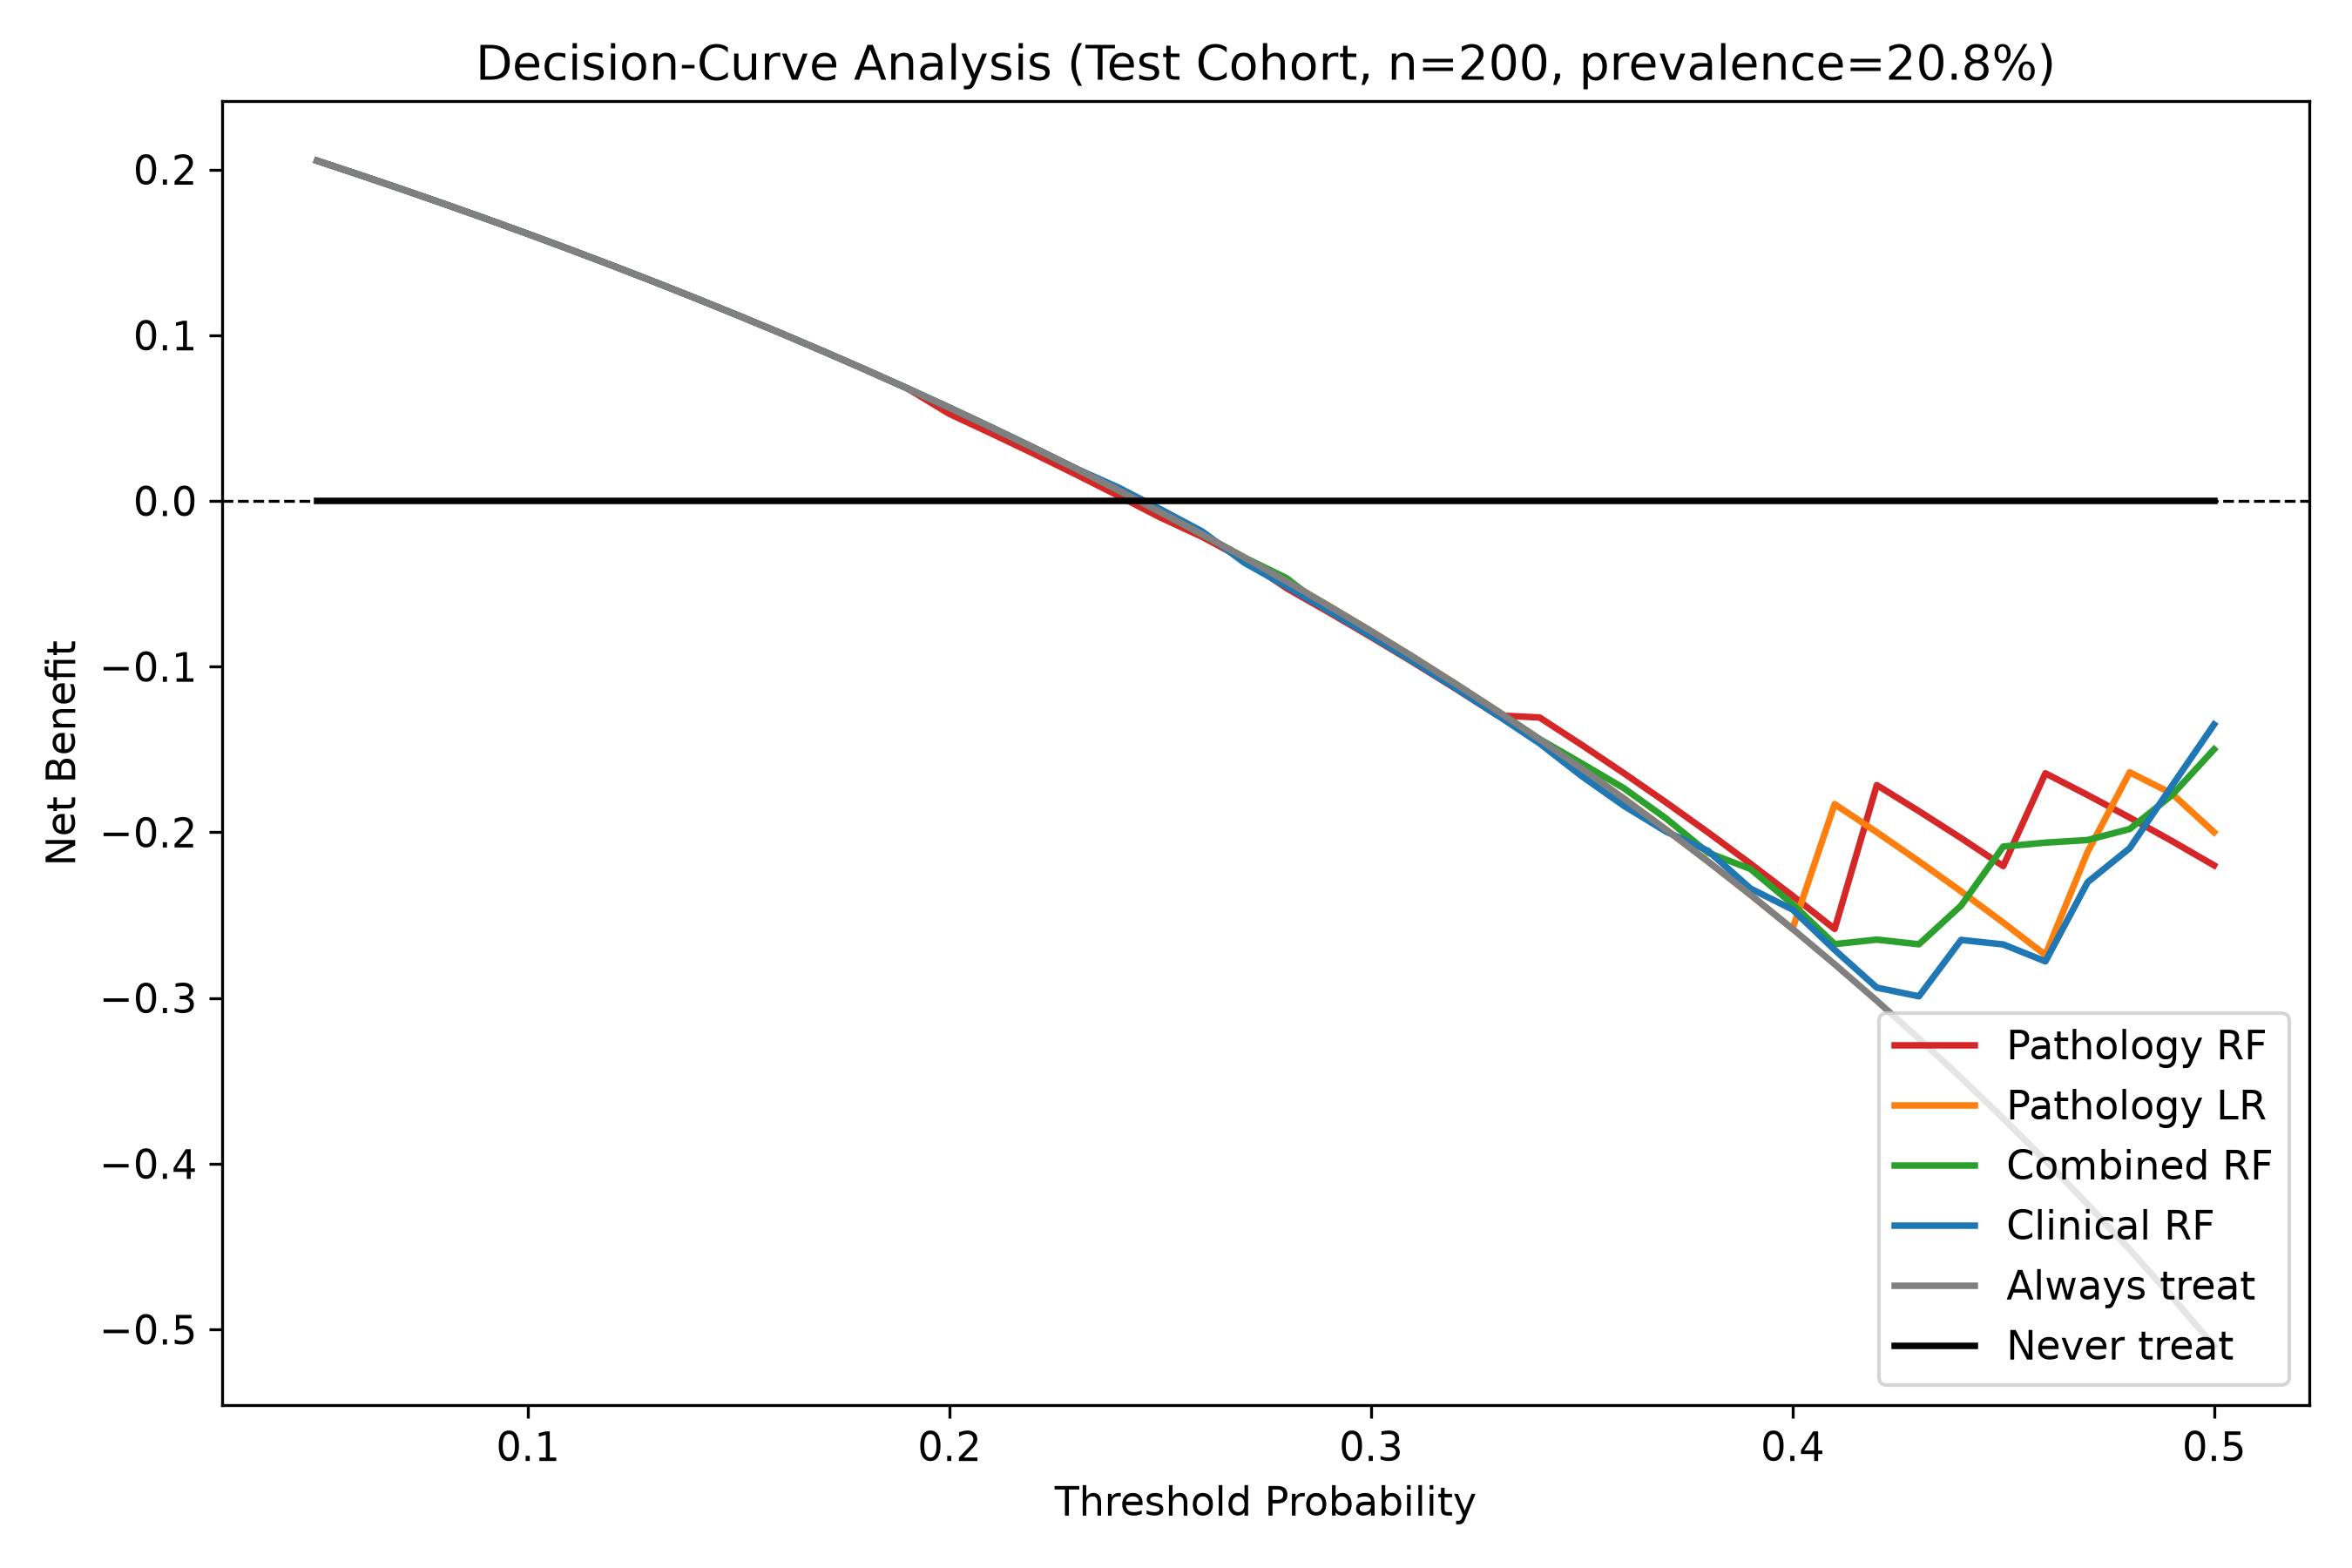
\includegraphics[width=\linewidth]{decision_curve_analysis.png}

    \column{0.48\textwidth}
      \begin{block}{Net Benefit Principle}
        $$\text{Net Benefit} = \frac{\text{TP}}{N} - \frac{\text{FP}}{N} \left(\frac{p_t}{1 - p_t}\right)$$
        Weighs benefit of detecting recurrence against burden of false-positive alarms across threshold $p_t$.
      \end{block}

      \begin{exampleblock}{Clinical Actionability Boundary}
        \begin{itemize}\setlength{\itemsep}{2pt}
          \item Pathology RF yields positive Net Benefit over standard strategies (``Treat All'' vs ``Treat None'') \textbf{only} in the narrow range:
          $$\mathbf{p_t \in [0.20, 0.35]}$$
          \item \textbf{Clinical Implication}: Viable for \textit{low-harm, non-invasive surveillance} (e.g. tighter imaging frequency), but \textbf{not} for high-toxicity adjuvant re-interventions.
        \end{itemize}
      \end{exampleblock}
  \end{columns}
\end{frame}

% ------------------------------------------------------------------------------
% SLIDE 11: DISCUSSION & STUDY LIMITATIONS (9:15 - 9:50)
% ------------------------------------------------------------------------------
\begin{frame}{Methodological Discussion \& Study Limitations}
  \begin{columns}[t]
    \column{0.50\textwidth}
      \begin{block}{Methodological Lessons}
        \begin{itemize}\setlength{\itemsep}{3pt}
          \item \textbf{Etiology vs. Progression}: Lifestyle carcinogens drive tumor genesis; intrinsic cellular differentiation drives post-surgical recurrence.
          \item \textbf{Statistical Association $\neq$ ML Power}: TD is statistically robust ($p=0.0022$), yet tabular ML discrimination remains moderate ($\ROC = 0.627$).
          \item \textbf{Curse of Tabular Sparsity}: 4 categorical pathology fields miss spatial histologic architecture (cellular stroma, tumor-infiltrating lymphocytes).
        \end{itemize}
      \end{block}

    \column{0.50\textwidth}
      \begin{alertblock}{Critical Study Limitations}
        \begin{itemize}\setlength{\itemsep}{2pt}
          \item \textbf{Test Event Ceiling}: Held-out test set has 49 events $\implies$ wide bootstrap intervals ($\ROC \in [0.528, 0.724]$).
          \item \textbf{Excluded HPV Status}: $22.4\%$ missing values prevented evaluating viral oncogenesis.
          \item \textbf{Uncalibrated Probability Output}: Balanced class weights shifted probabilities; recalibration required before prospective trial.
          \item \textbf{Single-Center Retrospective Design}: External multicenter cohort validation strictly required.
        \end{itemize}
      \end{alertblock}
  \end{columns}
\end{frame}

% ------------------------------------------------------------------------------
% SLIDE 12: CONCLUSION & PERSPECTIVES (9:15 - 10:00)
% ------------------------------------------------------------------------------
\begin{frame}{Conclusion \& Future Perspectives}
  \begin{columns}[c]
    \column{0.55\textwidth}
      \begin{block}{Key Scientific Takeaways}
        \begin{enumerate}\setlength{\itemsep}{3pt}
          \item \textbf{Timing Matters}: Surgical pathology is post-operative; clinical-only pre-op models show weak recurrence signal ($\ROC \approx 0.535$).
          \item \textbf{Pathology Drives Prognosis}: Tumor Differentiation is the primary independent predictor ($\aOR = 1.387, p=0.0022$).
          \item \textbf{Pathology RF reaches $\ROC = 0.627$}, but requires strict threshold management due to false-alarm costs.
        \end{enumerate}
      \end{block}

      \begin{exampleblock}{Future Research Perspectives}
        \begin{itemize}\setlength{\itemsep}{2pt}
          \item \textbf{Multimodal Integration}: Fusion of tabular clinical data with deep Whole-Slide Histopathology (WSI) features.
          \item \textbf{Isotonic Recalibration} \& multicentric prospective clinical evaluation.
        \end{itemize}
      \end{exampleblock}

    \column{0.45\textwidth}
      \begin{alertblock}{Clinical Translation Summary}
        \begin{itemize}\setlength{\itemsep}{2pt}
          \item Tabular models serve as \textbf{exploratory risk stratification} tools.
          \item Viable for \textbf{intensified non-invasive surveillance}, not for uncalibrated aggressive adjuvant therapies.
        \end{itemize}
      \end{alertblock}
  \end{columns}
\end{frame}

% ------------------------------------------------------------------------------
% SLIDE 13: CLOSING & Q&A (10:00)
% ------------------------------------------------------------------------------
\begin{frame}[plain]
  \centering
  \vspace{0.8cm}
  \begin{beamercolorbox}[sep=12pt,rounded=true,center,shadow=true]{title}
    {\Large \textbf{Thank You for Your Attention!}}\\[0.4cm]
    {\normalsize Questions \& Discussion with the Examination Jury}
  \end{beamercolorbox}
  
  \vspace{0.6cm}
  
\includegraphics[height=1.8cm]{logo.png}\\[0.3cm]
  {\footnotesize \textbf{Sultan Moulay Slimane University} -- Faculty of Sciences and Techniques of Béni Mellal}\\
  {\scriptsize Statistics \& Data Analysis Modules $\cdot$ Oral Defense -- Session C01-2}
\end{frame}

% ==============================================================================
% APPENDIX / BACKUP SLIDES (Outside 10-Min Talk - Dedicated Jury Q&A Support)
% ==============================================================================
\appendix

% ------------------------------------------------------------------------------
% BACKUP SLIDE A1: TEAM CONTRIBUTIONS (CRediT TAXONOMY)
% ------------------------------------------------------------------------------
\begin{frame}[noframenumbering]{Backup: Team Member Contributions (CRediT Taxonomy)}
  \begin{beamercolorbox}[sep=3pt,rounded=true,center]{block title}
    \textbf{Multidisciplinary Research Team -- Individual Contributions}
  \end{beamercolorbox}
  \vspace{0.15cm}

  \scriptsize
  \begin{tabular}{@{}p{2.8cm} p{2.6cm} p{9.0cm}@{}}
    \toprule
    \textbf{Member / Student} & \textbf{Discipline / Lab} & \textbf{Specific Project Contributions} \\
    \midrule
    \textbf{Yassine Oulhammous} & Artificial Intelligence \newline (Lab. TIAD) & Probabilistic calibration analysis (Brier score, logistic intercepts); operational threshold tuning (validation F1); Decision Curve Analysis (DCA); figure generation \& verification audit. \\
    \midrule
    \textbf{Mahdi Boughrous} & Artificial Intelligence \newline (Lab. TIAD) & Machine learning pipeline architecture; scikit-learn preprocessing \& one-hot encoding; LR and Random Forest model training; benchmark metric evaluation ($\ROC$, $\AUPRC$); \LaTeX{} lead. \\
    \midrule
    \textbf{Yasmine Elasri} & Mathematics \newline (Lab. MPA) & Statistical modeling pipeline; non-parametric hypothesis testing (Mann--Whitney $U$, $\chi^2$, Cramér's $V$); multivariable logistic regression \& odds ratios derivation; bootstrap CIs. \\
    \midrule
    \textbf{Mohamed Taha Benhassoun} & Biology & Biological and clinical scoping; oral cavity oncology synthesis; evaluation of lifestyle carcinogens (tobacco, alcohol, betel quid) vs recurrence; clinical interpretation. \\
    \midrule
    \textbf{Mustapha Amarzoug} & Organic Chemistry \newline (Lab. 3BIO) & Biochemical literature review; investigation of chemical carcinogens and cellular microenvironment factors; verification of biological plausibility \& critical review. \\
    \bottomrule
  \end{tabular}

  \vspace{0.15cm}
  {\tiny \textbf{Academic Supervision}: \textbf{Prof.~Aziz OUHINOU} \& \textbf{Prof.~Hicham MOUSSA} (FST Béni Mellal, USMS).}
\end{frame}

% ------------------------------------------------------------------------------
% BACKUP SLIDE A2: SECONDARY ANALYSES & UNCERTAINTY AUDIT
% ------------------------------------------------------------------------------
\begin{frame}[noframenumbering]{Backup: Statistical Uncertainty \& Sensitivity Audit}
  \begin{columns}[t]
    \column{0.55\textwidth}
      \begin{block}{\scriptsize Secondary Analyses on Held-Out Test ($n=200$, 49 events)}
        \centering
        \tiny
        \begin{tabular*}{\linewidth}{@{\extracolsep{\fill}}llcl@{}}
          \toprule
          \textbf{Analysis} & \textbf{Model} & \textbf{Result} & \textbf{Detail / 95\% CI} \\
          \midrule
          Bootstrap $\ROC$ & Pathology RF & 0.627 & [0.528, 0.724] (1\,000 resamples) \\
          Bootstrap $\AUPRC$ & Pathology RF & 0.406 & [0.286, 0.547] \\
          Paired AUC Diff & Path RF vs Comb RF & +0.069 & [$-0.018$, 0.160] (CI includes 0) \\
          Seed Robustness & Pathology RF & 0.627--0.633 & Seeds 2024, 42, 123 \\
          \midrule
          Threshold 0.50 & Pathology RF & Recall 0.633 & 31 TP, 75 FP, 76 TN, 18 FN \\
          Threshold 0.453 & Pathology RF & Recall 0.837 & 41 TP, 104 FP, 47 TN, 8 FN \\
          \bottomrule
        \end{tabular*}
      \end{block}

    \column{0.45\textwidth}
      \begin{alertblock}{\scriptsize Methodological Insights for Q\&A}
        \begin{itemize}\setlength{\itemsep}{1pt}
          \item {\tiny \textbf{Pairwise Non-Significance}: The observed AUC advantage of Pathology RF over Combined RF (+0.069) has a 95\% CI spanning zero $\implies$ difference is not statistically confirmed.}
          \item {\tiny \textbf{Seed Stability}: Performance across alternative initializations (seeds 42, 123, 2024) remains tightly bounded within $[0.627, 0.633]$.}
        \end{itemize}
      \end{alertblock}
  \end{columns}
\end{frame}

\end{document}
